\documentclass[conference]{IEEEtran}
\IEEEoverridecommandlockouts
% The preceding line is only needed to identify funding in the first footnote. If that is unneeded, please comment it out.
\usepackage{cite}
\usepackage{amsmath,amssymb,amsfonts}
\usepackage{algorithmic}
\usepackage{fixltx2e}
\usepackage{graphicx}
\usepackage{textcomp}
\usepackage{xcolor}
\usepackage[clean]{svg}
\usepackage{amsmath}
\usepackage{graphicx}
\usepackage{float}
\usepackage{pifont}
\usepackage{multirow}
\def\BibTeX{{\rm B\kern-.05em{\sc i\kern-.025em b}\kern-.08em
    T\kern-.1667em\lower.7ex\hbox{E}\kern-.125emX}}
\begin{document}

\title{Step Detection Based on Artificial Neural Networks
}

\author{\IEEEauthorblockN{Bernardo Costa, Fábio Almeida, Ivo Rodrigues
}
\IEEEauthorblockA{Department of Electronics, Telecommunications and Informatics, University of Aveiro, Portugal}
\IEEEauthorblockA{Fundamentals of Machine Learning (Prof. Petia Georgieva)}
}

\maketitle
\thispagestyle{plain}
\pagestyle{plain}

\begin{abstract}
The present work aims to discuss the implementation of a step detection algorithm using an Artificial Neural Network (ANN), through binary classification according to the provided smartphone accelerometer data.
\end{abstract}

\begin{IEEEkeywords}
machine learning, artificial neural networks, step detection, algorithms.
\end{IEEEkeywords}

\section{Introduction}
The motivation for this step detection algorithm came during an ongoing MSc thesis project entitled "Practice as you walk", a smartphone application aiming to aid young musicians to improve their musical skills by extending their practice hours.\par
Most step detection algorithms only attain acceptable accuracy with a very high latency, due to the processing-intensive nature of the typically employed algorithms. It was our goal to develop a simpler mechanism for step detection, with the help of Machine Learning (ML), through ANNs.\par
One of the main benefits of this approach is that it might even allow, in the future, for the users to train the employed model with their own data. 

\section{Data description and preprocessing}
The application for raw data logging requires the smartphone to be held in the texting position, such as shown in figure 1, since the main application being developed in the MSc project is supposed to continuously interact with the user. \par
Therefore, the only relevant data to be collected (due to the average smartphone position) is the acceleration along the Z axis, provided by the accelerometer sensor.

\begin{figure}[H]
    \centering
    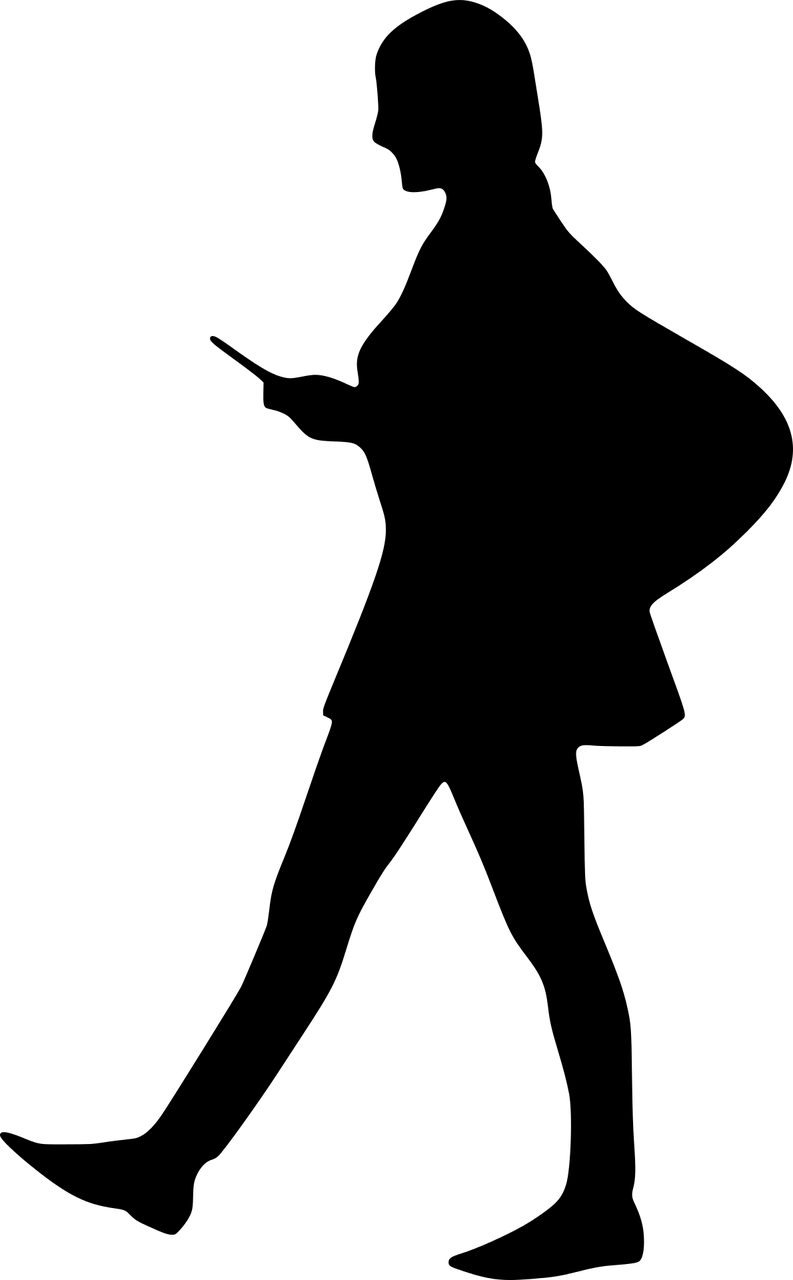
\includegraphics[scale=0.1]{woman-2803967_1280.png}
    \caption{A woman holding a smartphone in the texting position}
    \label{fig:wom_smartphne}
\end{figure}

Both training and testing data are acquired via the accelerometer sensor of a Samsung Galaxy A80 smartphone, through an Android application developed in Unity. The ground truth, corresponding to real step occurrences, is given by the user (figure 2) when the blue button is pressed. 



\begin{figure}[H]
\centering
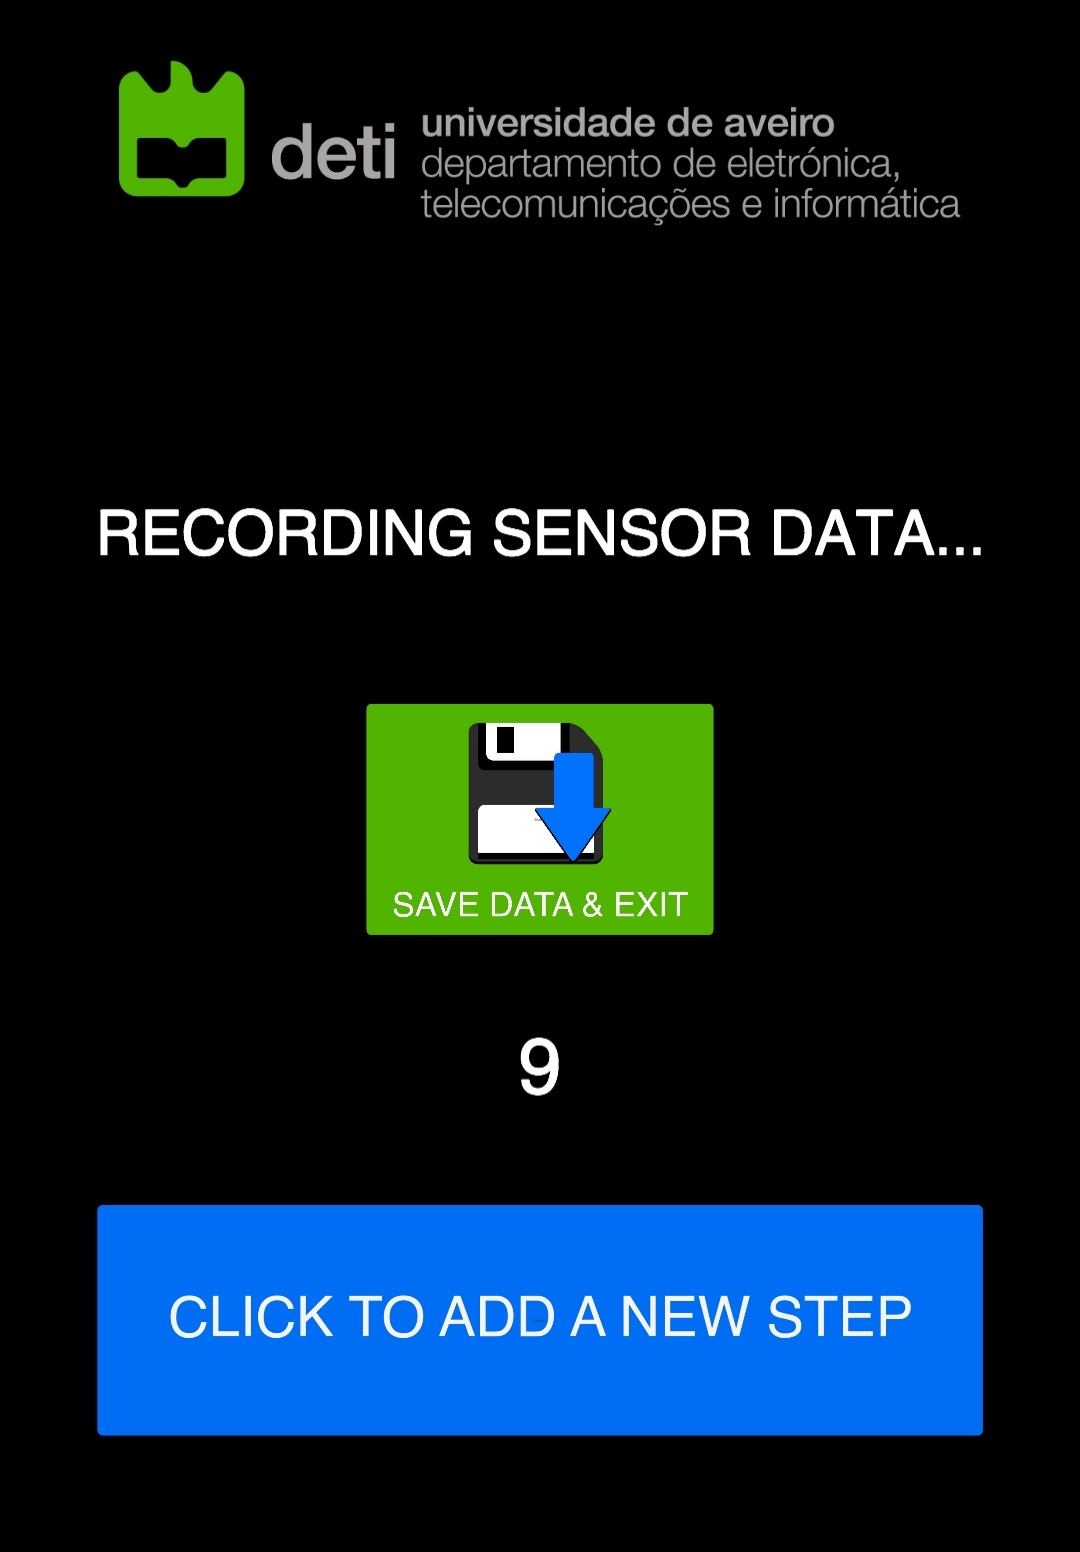
\includegraphics[scale=0.1]{Screenshot_Steps.jpg}
\caption{Cropped screen capture of the mobile app}
\label{fig:app}
\end{figure}

Initially, the data acquisition ran at the sampling frequency of 60 Hz, as imposed by the Unity Engine (display refresh rate of the smartphone).\par
The user would press the button when their feet hit the floor, signaling the occurrence of a step, which would return a single '1' to the ground truth vector, with the non-steps being represented by '0's.\par
However, two problems were immediately identified:

\begin{itemize}
    \item this sampling frequency resulted in the acquisition of unwanted high-frequency events;
    \item the data was naturally unbalanced, due to the massive occurrence of non-steps in the data set.
\end{itemize}

In order to mitigate both issues, the sampling rate was reduced to 10Hz, via down-sampling, since most relevant information peaked around 5Hz (with respect to the Nyquist theorem); furthermore, every step signaled by the user results in three consecutive '1's, accounting for the user's natural reaction time and the averaging of valid step samples.\par
Essentially, this resulted in clearer data with no unwanted interference and naturally more balanced.
\par The smartphone application finally exports the logged data when the green button is pressed; this information was then imported to a MATLAB script for processing, plotting and detailed inspection purposes.\par
The raw accelerometer data, as well as the differences between accelerometer samples and the ground truth provided by the user can be observed in figures 3 and 4.
\begin{figure}[H]
\centering
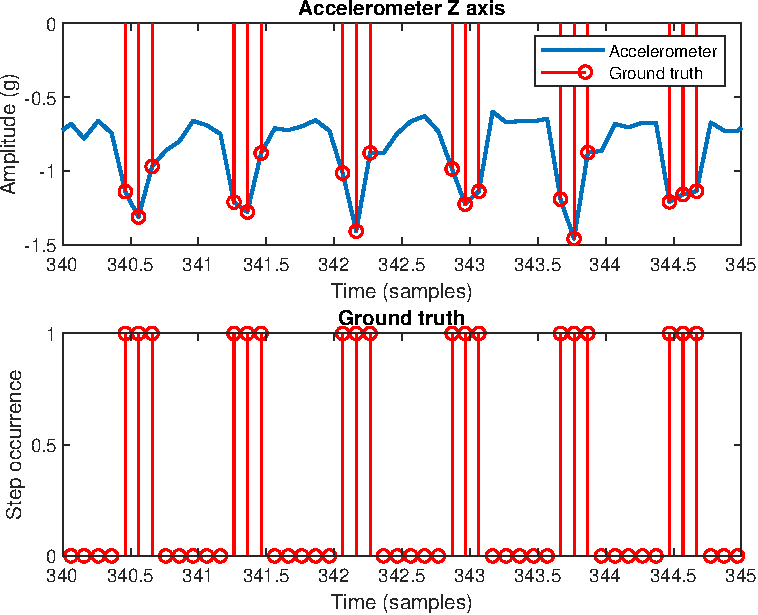
\includegraphics[scale=0.6]{Figure1.pdf}
\caption{Raw accelerometer data (Z axis)}
\label{fig:rawacc}
\end{figure}
\begin{figure}[H]
\centering
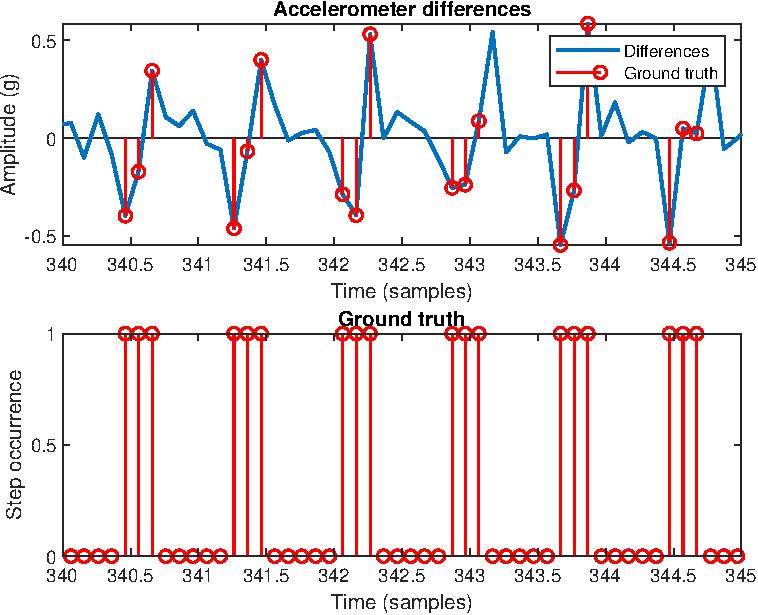
\includegraphics[scale=0.6]{Figure2.pdf}
\caption{Raw accelerometer differences}
\label{fig:rawdif}
\end{figure}

As observable, the behavior of the acquired data when nearing a step occurrence is highly dynamic; while it might seem that a simple threshold would suffice for this particular application, there are step occurrences with low amplitudes.
\par Therefore, the data was reformatted so that step windows of select features (figure 5) are considered, instead of individual samples with no specific meaning.\par
\begin{figure}[h]
\centering
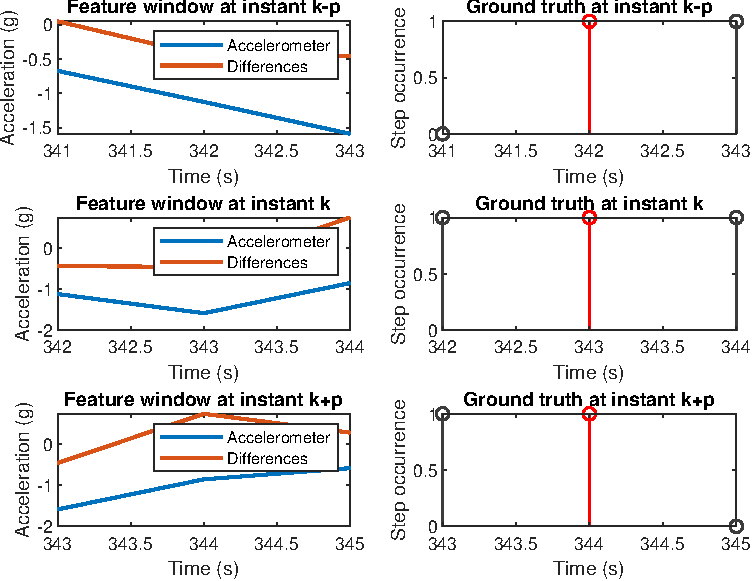
\includegraphics[scale=0.6]{Figure3.pdf}
\caption{Reformatted six-feature windows}
\label{fig:wind}
\end{figure}

These features consist of: 
\begin{itemize}
    \item a window containing accelerometer (Z axis) samples corresponding to the time interval: ${[}k-p,k+p{]}$;
    \item a window containing the differences between the accelerometer samples at instants ${}k-1$ and $k$.
\end{itemize}

Additionally, some examples of non-steps were removed from the data set in order to achieve 50/50 balance between step and non-step examples. \par This new structure allows for the ANN model to understand the weights of each sample for the correct detection of steps, essentially making the system aware of dynamics.\par

\section{Logistic regression model}
While apparently not fit for a regression approach, the main objective of this problem is to achieve binary classification based on feature weighting, meaning even a simple, non-regularized logistic regression model could actually perform very well under the new windowed version of the data set.  \cite{b6} \par

\subsection{Definition}
Logistic regression is a classification method able to match observations to a discrete set of classes. Unlike linear regression, which outputs continuous values, logistic regression uses the sigmoid function to return a probability value. This value can then be mapped to two or more discrete classes.

\subsection{Sigmoid function}\label{SIGFUN}
The sigmoid function\cite{b2} is a special form of the logistic function, given by:
\begin{equation}
    \sigma(x) = \frac{1}{(1+e^{-x})}
    \label{eq1}
\end{equation}
\par Also called a squashing function, the domain of the sigmoid function is the set of all real numbers, while its range is (0, 1). Therefore, in machine learning, the sigmoid function is used as an activation function, to map predictions to probabilities.

\subsection{Cost function and gradient}
The logistic regression model is defined as: 
\begin{equation}
    h_{\theta}(x^{(i)})=  \frac{1}{1+e^{-\theta (x^{(i)})}}
    \label{eq2}
\end{equation}
\par In logistic regression, the cost function, which is a measure of how wrong the model can estimate the relationship between its inputs and outputs, is given by:
\begin{equation}
    J(\theta) = \frac{1}{m} \sum_{i=1}^{m} [ -y^{(i)}log(h_{\theta}(x^{(i)})) - (1 - y^{(i)})log(1 - (h_{\theta}(x^{(i)}))]
    \label{eq3}
\end{equation}
\par The gradient (generalization of the derivative for multivariate functions) of $J(\theta)$ is a vector of the same length as $\theta$,  where the $j_{th}$ element (for $j = 0, 1, ..., n$) is defined as:
\begin{equation}
    \frac{\partial J(\theta)}{\partial \theta_j} = \frac{1}{m} \sum_{i=1}^{m} (h_{\theta}(x^{(i)}) - y^{(i)})x_j^{(i)}
    \label{eq4}
\end{equation}

\subsection{Feature normalization}
In this case, since the features (accelerometer data and respective differences) are in the same order of magnitude, there is no need to perform mean normalization.

\subsection{Gradient descent}
Gradient descent is an optimization algorithm used to minimize a cost function, by iteratively moving in the direction of steepest descent. In our particular case, the minimization of the cost function $J(\theta)$ is done by updating the equation below (simultaneously updating $\theta_j$ for all $j$), at the rate specified by $\alpha$ (learning rate), and repeating until convergence.    
\begin{equation}
    \theta_j := \theta_j - \alpha \frac{1}{m} \sum_{i=1}^m (h_{\theta}(x^{(i)}) - y^{(i)})x_j^{(i)}
    \label{eq5}
\end{equation}
\par For the logistic regression model, the hypothesis $h_{\theta}(x)$ is the sigmoid function:
\begin{equation}
    h_{\theta}(x)= \frac{1}{1+e^{-\theta^T x}}
    \label{eq6}
\end{equation}


\subsection{Performance metrics for the logistic regression model}
Effectively, 400 iterations of the gradient descent, for learning rates greater than or equal to 0.1, were enough to make a basic logistic regression model converge to the minimum cost, as can be seen in figure 6. 
\begin{figure}[H]
\centering
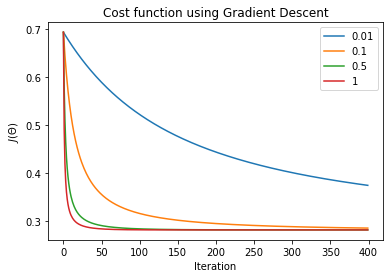
\includegraphics[scale=0.6]{LOGREG.png}
\caption{Cost function for the logistic regression model}
\label{fig:logregcost}
\end{figure}

The model could be further improved through regularization of the cost function; however, the logistic regression model is only intended, in this context, as a comparison to the main objective of this project: the artificial neural network.

\par Still, the accuracy of the training (although not an effective performance metric for this particular problem, due to the downside of fake and undetected steps) peaked at 88.73\% for the training set and at 88.25\% for the testing set, considering a decision threshold of 0.5. \par Regarding individual situations, the model attained correspondences of up to 99.95\% when the input was an ideal step window and down to 0.5\% with an ideal non-step window. \par

A sturdy performance metric is the $F1$ score, a weighted average of $Precision$ and $Recall$; these terms are based on the occurrence of true positives ($TP$) and true negatives ($TN$), as well as false positives ($FP$) and false negatives ($FN$). \par

As such, $Precision$ and $Recall$ are calculated as below:
\begin{equation}
    Precision = \frac{TP}{TP+FP}
    \label{eq7}
\end{equation}
\begin{equation}
    Recall = \frac{TP}{TP+FN}
    \label{eq8}
\end{equation}

For the $F1$ score, considering the testing data set, the achieved results are shown in the confusion matrix below:
\begin{table}[H]
\centering
\caption{Confusion matrix (logistic regression)}
\label{tab:my-table}
\begin{tabular}{cccc}
                                       &                       & \multicolumn{2}{c}{Predicted}                          \\ \cline{3-4} 
                                       & \multicolumn{1}{c|}{} & \multicolumn{1}{c|}{Positive} & \multicolumn{1}{c|}{Negative} \\ \cline{2-4} 
\multicolumn{1}{c|}{\multirow{2}{*}{Real}} & \multicolumn{1}{c|}{Positive} & \multicolumn{1}{c|}{519} & \multicolumn{1}{c|}{81} \\ \cline{2-4} 
\multicolumn{1}{c|}{}                  & \multicolumn{1}{c|}{Negative} & \multicolumn{1}{c|}{79} & \multicolumn{1}{c|}{708} \\ \cline{2-4} 
\end{tabular}
\end{table}
\par Then, $Precision$, $Recall$ and the $F1$ score are calculated:
\begin{equation}
    Precision = \frac{519}{519+79} = 86.8\%
    \label{eq9}
\end{equation}
\begin{equation}
    Recall = \frac{519}{519+81} = 86.5\%
    \label{eq10}
\end{equation}
\begin{equation}
    F1 = 2 \cdot \frac{Recall \cdot Precision}{Recall+Precision} = \frac{86.5\% \cdot 86.8\%}{86.5\%+86.8\%} = 86.6\%
    \label{eq11}
\end{equation}



\section{Artificial Neural Network}
The main objective here was to develop an ANN that could outperform the previous logistic regression model. 

\subsection{Definition}\label{ANNdef}
Artificial Neural Networks are computational models inspired by the biological neural networks present in animals. 
\par In machine learning, these networks correspond to a collection of connected computational nodes (neurons), which are arranged in multiple computational layers.

\subsection{Structure}
The first thing to do is to idealize the dimensions (number of inputs, number of hidden layers, size of the hidden layers and number of outputs) of our ANN, based on the standard structure shown in figure 7.

\begin{figure}[H]
\centering
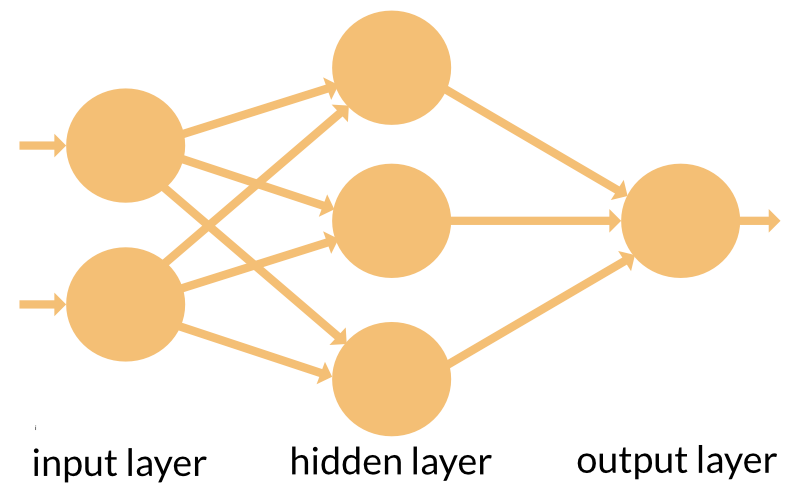
\includegraphics[scale=0.25]{ANNstruct.png}
\caption{Basic structure of an ANN with a single hidden layer}
\label{fig7}
\end{figure}

For our ANN, the size of the input layer (number of inputs) is naturally six, as determined by the number of features on our data sets (the step windows). 
\par
The number of hidden layers is associated with the desired result for our model, especially in terms of their performance depending on linearity:
\begin{itemize}
    \item a network with no hidden layers is only capable of representing linearly separable functions or decisions;
     \item a single hidden layer can approximate any function of continuous mapping from one finite space to another;
     \item two hidden layers can represent an arbitrary decision boundary to arbitrary accuracy with rational activation functions, being able to approximate any smooth mapping to any accuracy;
     \item more than two hidden layers allow for the model to learn complex representation (high computational resources, as in deep learning).
\end{itemize}
\par Considering our particular case, the computational cost of more than a single hidden layer would not bring any benefits, as the capabilities of a single layer are more than enough for the structure of our data set and corresponding outputs, as shown previously by the relatively good performance of the logistic regression model. One parameter that is of higher importance for this ANN is the size of this single hidden layer.
\par The size of a single hidden layer, as a rule of thumb, should be somewhere between the size of the input layer and the size of the output layer. Therefore, through a cross-validation (CV) method (approached further in this report) with the size varying between 1 (size of the output layer) and 6 (size of the input layer), result improvements ceased after a hidden layer size of 3, which ended up being the selected value.
\par Finally, the size of the output layer (number of outputs) is 1, as the intended results are of binary classification nature.

\subsection{Cost function}
The non-regularized cost function for this ANN (binary classification) is the same as the logistic regression cost function in equation 3. The regularized cost function is obtained through just the addition of the regularization term:
\begin{equation}
    J(\theta)_{reg} = J(\theta)+ \frac{\lambda}{2m}\sum_{j=1}^n \theta_{j}^2
    \label{eq12}
\end{equation}

\subsection{Gradient descent and error back-propagation}
In a very similar way to the previously mentioned gradient descent, the model learns iteratively by minimizing the error between the predicted values and the ground truth; however, considering there is a hidden layer whose features are unknown to the user, there needs to be a way to understand how much every hidden feature is responsible for the current error.
\par This is exactly what is known as error back-propagation \cite{b4}: the output error of the ANN is analysed so that the weight of each feature can be adjusted in order to minimize that error; the standard sequence for error back-propagation is as follows:


\begin{itemize}
    \item 1) randomly initialize the parameters ($\Theta_1$ and $\Theta_2$);
    \item 2) for $i = 1:num_{examples}$ iteration begin:
    \item 3) provide training example $i$ at the NN input;
    \item 4) perform a feedforward pass (figure 8) to compute $z^{(2)}$, $a^{(2)}$ (for the hidden layer) and
$z^{(3)}$, $a^{(3)}$ (for the output layer);

\end{itemize}

\begin{figure}[H]
\centering
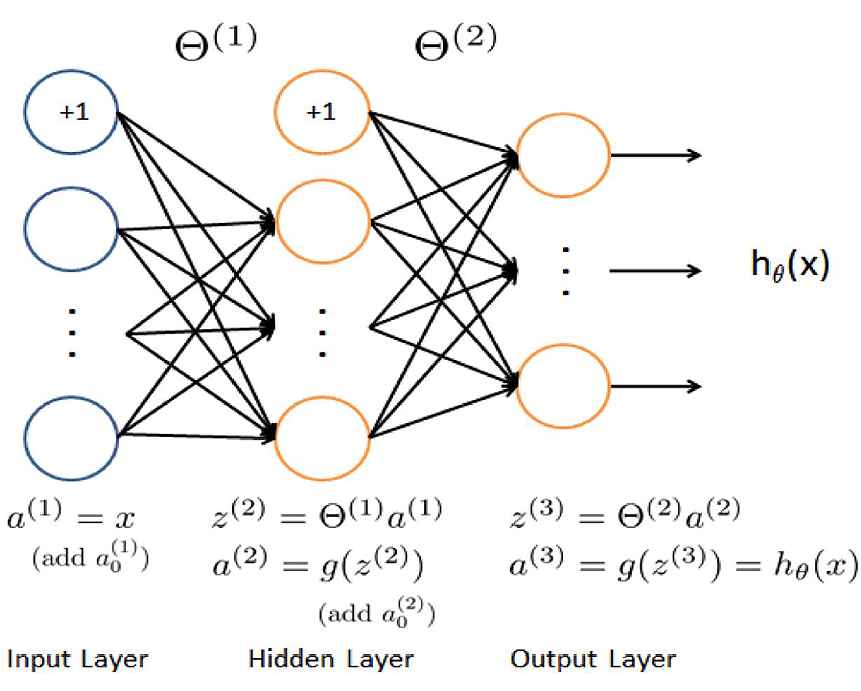
\includegraphics[scale=0.4]{ann_eq_n.png}
\caption{ANN model learning: forward pass}
\label{fig8}
\end{figure}

\begin{itemize}
    \item 5) for each unit k in the output layer compute: $z^{(2)}$, $a^{(2)}$ (hidden layer) and
$z^{(3)}$, $a^{(3)}$ (output layer);
    \begin{equation}
    \delta^{(3)}_k = (a^{3}_k - y_k) 
    \label{eq13}
    \end{equation}
    \item 6) for the hidden layer, compute: 
    \begin{equation}
    \delta^{(2)} = (\Theta^{2})^{T}\delta^{3}.g'(z^{2})
    \label{eq14}
    \end{equation}
    \item 7) accumulate the gradient from this example:
    \begin{equation}
    \Delta^{(l)} = \Delta^{l}+\delta^{(l+1)}(a^{l})^{T}
    \label{eq15}
    \end{equation}
    \item 8) NN gradient (no regularization):
    \begin{equation}
     \frac{\partial J(\theta)}{\partial \theta_{ij}^{(l)}} = \frac{1}{m} \Delta_{ij}^{(l)}
    \label{eq16}
    \end{equation}
    \item 9) update NN parameters:
    \begin{equation}
    \Theta_{ij}^{(l)} = \Theta_{ij}^{(l)} -\alpha \frac{\partial J(\theta)}{\partial \theta_{ij}^{(l)}}
    \label{eq17}
    \end{equation}
    \item 10) iteration end.
\end{itemize}

\subsection{Activation functions}
For this ANN, two versions were approached: one with the sigmoid as the activation function of the hidden layer, and other with the leaky-ReLU function, presented in the next section. The activation function for the output layer is always the sigmoid function, which returns values between 0 and 1.

\subsection{Leaky-ReLU function and gradient}
The leaky-ReLU function\cite{b3} is a type of activation function based on rectified linear units. This function is a variation of the ReLU function, with a small positive slope, in the negative area, in order to enable back-propagation even for negative input values. 
\begin{equation}
\centering
    f (x) = 
    \begin{cases}
      \alpha x   , x \leq 0 \\
      x ,  x > 0
    \end{cases}\,
\end{equation}

The derivative of this function is as follows:
\begin{equation}
    f'(x) = 
    \begin{cases}
      \alpha   , x \leq 0 \\ 
      1 ,  x > 0
    \end{cases}\,
\end{equation}

\subsection{K-folds cross-validation}
The cost function regularization parameter $\lambda$ should not be chosen freely; instead, a systematic approach was chosen: through the K-folds CV method, the best value for $\lambda$ is calculated.
\par The k-folds CV method consists on splitting the data set into two subsets (training data and test data); then, the training data is split in $K$ subsets (folds). This method uses $K-1$ folds to train the model and the remaining fold to cross-validate the model. Since we have $K$ folds, the algorithm iterates over $K$ different iterations\cite{b6}, as shown in figure 9.\cite{b5} 
\begin{figure}[H]
\centering
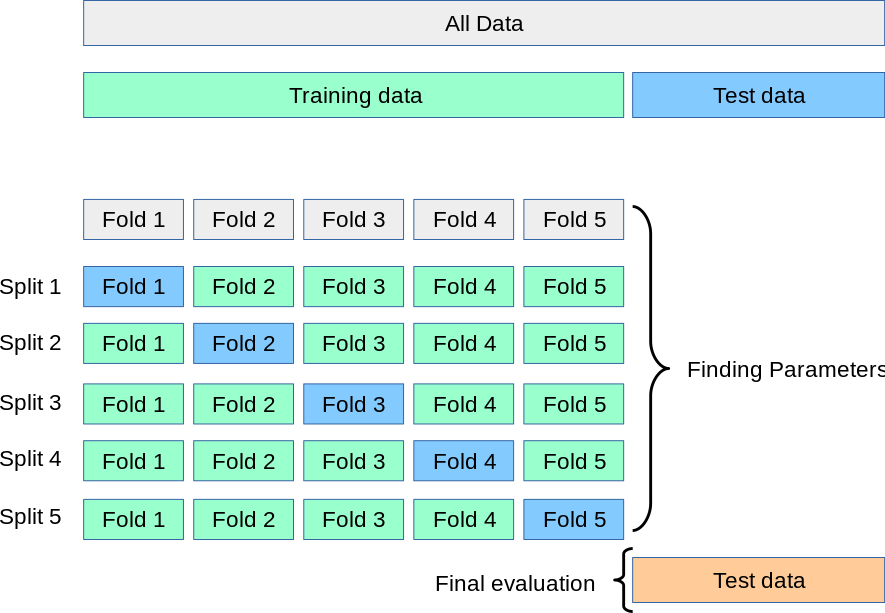
\includegraphics[scale=0.25]{kfolds.png}
\caption{K-folds CV algorithm}
\label{fig:kfolds}
\end{figure}

\par At the end of all iterations, a CV error is calculated based on the mean of the sum of all iteration errors.


\subsection{Hyper-parameter selection}
With almost all the parameters of the ANN chosen we use the K-folds CV method in order to determine the best hyper parameter $\lambda$. As mentioned before, we used two different activation functions. The first was the sigmoid function, with a total of 1000 iterations and $\alpha$=1. The cost function of the K-folds CV method over the iterations, for the different $\lambda$ values, is shown below:

\begin{figure}[H]
\centering
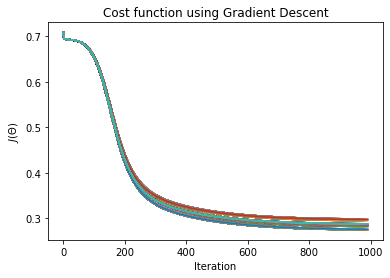
\includegraphics[scale=0.6]{CostFuncEvo.png}
\caption{Cost function over K-folds iterations and different $\lambda$ values}
\label{fig:kfoldsiter}
\end{figure}

\par
At the end of this process, a best $\lambda$ of value 0 was obtained (this was also the case for the leaky-ReLU version). 

\subsection{Performance metrics for the ANN model: sigmoid version}
With all hyper-parameters correctly defined, the model was trained with the training set and obtained a training accuracy of 89.66\% for a 0.49 decision threshold. For the testing set, the accuracy peaked at 89\%, with a 0.73 decision threshold.
\par 
The cost function for the trained model with the best hyper-parameters can be observed in figure 11.
\begin{figure}[H]
\centering
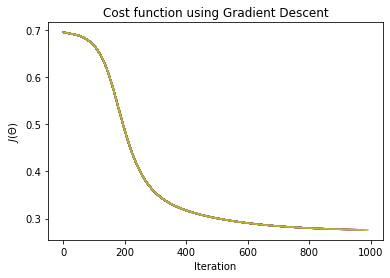
\includegraphics[scale=0.6]{CostFuncTrainSigm.png}
\caption{Cost function for best hyper parameters}
\label{fig:kfoldsiter}
\end{figure}

\par
The confusion matrix for the testing set is as follows: 
\begin{table}[H]
\centering
\caption{Confusion matrix (ANN: sigmoid activation function)}
\label{tab:my-table}
\begin{tabular}{cccc}
                                       &                       & \multicolumn{2}{c}{Predicted}                          \\ \cline{3-4} 
                                       & \multicolumn{1}{c|}{} & \multicolumn{1}{c|}{Positive} & \multicolumn{1}{c|}{Negative} \\ \cline{2-4} 
\multicolumn{1}{c|}{\multirow{2}{*}{Real}} & \multicolumn{1}{c|}{Positive} & \multicolumn{1}{c|}{513} & \multicolumn{1}{c|}{87} \\ \cline{2-4} 
\multicolumn{1}{c|}{}                  & \multicolumn{1}{c|}{Negative} & \multicolumn{1}{c|}{45} & \multicolumn{1}{c|}{555} \\ \cline{2-4} 
\end{tabular}
\end{table}

\begin{equation}
    Precision = \frac{513}{513+45} = 91.9\%
    \label{eq9}
\end{equation}
\begin{equation}
    Recall = \frac{513}{513+81} = 85.5\%
    \label{eq10}
\end{equation}
\begin{equation}
    F1 = 2 \cdot \frac{Recall \cdot Precision}{Recall+Precision} = \frac{85.5\% \cdot 91.9\%}{85.5\%+91.9\%} = 88.6\%
    \label{eq11}
\end{equation}

\subsection{Performance metrics for the ANN model: leaky-ReLU version}
Similarly, the model was trained with the training data set, only this time with 1200 iterations and $\alpha$=0.2 . 
\par 
The training accuracy obtained for the training data was 89.76\% for a 0.45 decision threshold. For the testing set, the accuracy peaked at 88.41\%, with a 0.72 decision threshold.

The cost function for the trained model with the best hyper-parameters can be observed in figure 12.
\begin{figure}[H]
\centering
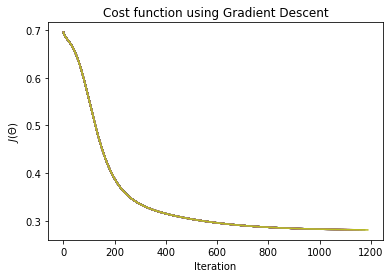
\includegraphics[scale=0.6]{CostFuncTrainLEAKYRELU.png}
\caption{Cost function for best hyper parameters}
\label{fig:kfoldsiter}
\end{figure}

\begin{table}[H]
\centering
\caption{Confusion matrix (ANN: leaky-ReLU activation function)}
\label{tab:my-table}
\begin{tabular}{cccc}
                                       &                       & \multicolumn{2}{c}{Predicted}                          \\ \cline{3-4} 
                                       & \multicolumn{1}{c|}{} & \multicolumn{1}{c|}{Positive} & \multicolumn{1}{c|}{Negative} \\ \cline{2-4} 
\multicolumn{1}{c|}{\multirow{2}{*}{Real}} & \multicolumn{1}{c|}{Positive} & \multicolumn{1}{c|}{513} & \multicolumn{1}{c|}{87} \\ \cline{2-4} 
\multicolumn{1}{c|}{}                  & \multicolumn{1}{c|}{Negative} & \multicolumn{1}{c|}{52} & \multicolumn{1}{c|}{548} \\ \cline{2-4} 
\end{tabular}
\end{table}

\begin{equation}
    Precision = \frac{513}{513+52} = 90.8\%
    \label{eq9}
\end{equation}
\begin{equation}
    Recall = \frac{513}{513+87} = 85.5\%
    \label{eq10}
\end{equation}
\begin{equation}
    F1 = 2 \cdot \frac{Recall \cdot Precision}{Recall+Precision} = \frac{85.5\% \cdot 90.8\%}{85.5\%+90.8\%} = 88.1\%
    \label{eq11}
\end{equation}

\section{Conclusions}
As expected, the ANN model outperforms the logistic regression model. However, the difference between the two models was much lower than the expected, and the results did not achieve a minimum of 90\% in any of the performance metrics.
\par In conclusion, while fit for step detection under a controlled environment, the ANN model is not yet what the previously referred MSc thesis project is looking for. Perhaps, in the future, a more advanced algorithm (probably based on deep learning) will achieve the desired results.

\section{Comparison with existing solutions}
A very interesting ML-based solution was developed by a Portuguese student (Rodrigues, G.) for their MSc thesis in Biomedical Engineering. \cite{b1}
\par Entitled "Real-Time Step Detection Using Unconstrained Smartphone", the original document describes and compares multiple ML-based algorithms and their applicability in the field of step detection. 
\par The author chose a deep learning model based on Convolutional Neural Networks, which attained results of the same order as ours (accuracies and F-scores not that higher) but much more consistent and reliable, due to the support of multiple smartphone positions.

\section{Work load per student}
\textbf{Bernardo Costa} - Responsible for collecting data (mobile app development), contribution in MATLAB data formatting, Python programming and writing the report; \par
\textbf{Fábio Almeida} - Contribution writing the algorithm, MATLAB data formatting, adapting the ANN model from class 4 (Python) to binary classification and writing the report; \par
\textbf{Ivo Rodrigues} - Contribution in Python programming, MATLAB data formatting, and writing the report.


\begin{thebibliography}{00}
\bibitem{b1} Gonçalo M. G. Rodrigues, "Real-Time Step Detection Using Unconstrained Smartphone", 2020
\bibitem{b2} Mehreen Saeed, "A Gentle Introduction To Sigmoid Function", machinelearningmastery.com, 2021
\bibitem{b3} Jason Brownlee, "A Gentle Introduction to the Rectified Linear Unit (ReLU)", machinelearningmastery.com, 2021
\bibitem{b4} James C.R. Whittington and Rafal Bogacz1, "Theories of Error Back-Propagation in the Brain", Trends in Cognitive Sciences, Vol. 23, No. , 2019
\bibitem{b5} "Cross-validation: evaluating estimator performance", scikit-learn.org, 2021
\bibitem{b6} Petia Georgieva, "Foundations of Machine Learning - Lecture 3: Classification: Logistic Regression", elearning.ua.pt, 2021
\bibitem{b7} Petia Georgieva, "Foundations of Machine Learning - Lecture 4: Neural Networks", elearning.ua.pt, 2021
\bibitem{b8} Petia Georgieva, "Foundations of Machine Learning - Lecture 5: Support Vector Machine (SVM)", elearning.ua.pt, 2021
\bibitem{b9} Petia Georgieva, "Foundations of Machine Learning - Lecture 6: Model Selection and Validation - Bias vs. Variance", elearning.ua.pt, 2021

\end{thebibliography}


\end{document}
